\documentclass{article}
\usepackage{geometry}
\usepackage{graphicx}
\usepackage{array}
\usepackage{longtable}
\geometry{margin=1in}
\begin{document}
This article documents my workflow of the WeBWork-Canvas integration. We assume the operating system is Windows 10.\footnote{Version 0.5}

\section{Enrolling Students in WeBWork}
In this section, we go over how to enroll students to a class on WeBWork based on a class on Canvas. The key step is to create a .lst file via the gradebook exported from Canvas.

{
\centering
\begin{longtable}{|l|l|}
\hline
\begin{parbox}{0.45\textwidth}{}
\end{parbox}&\begin{parbox}{0.45\textwidth}{
Download a copy of\\ WeBWork\_classlist\_template.xlsx. In the following, we refer to this file as {\bf the Template}.}
\end{parbox}\\
\hline
\begin{parbox}{0.45\textwidth}{
\centering
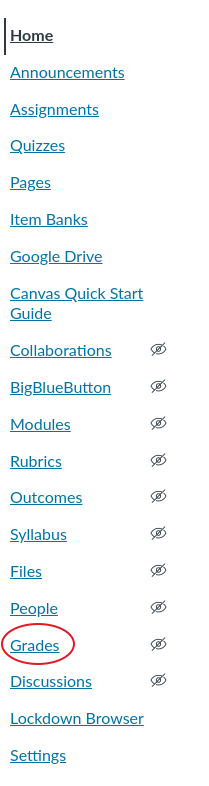
\includegraphics[width=.15\textwidth]{canvasNavbarGrade.png}}
\end{parbox}&\begin{parbox}{0.45\textwidth}{
In the course on Canvas you want to enroll the students from, click Grade from the navigation bar on the left.}
\end{parbox}\\
\hline
\begin{parbox}{0.45\textwidth}{\centering
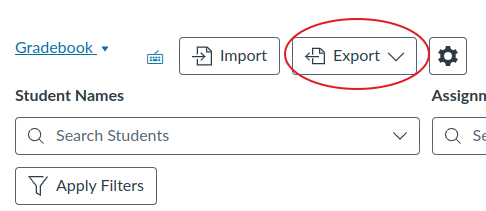
\includegraphics[width=.30\textwidth]{gradebookExport.png}}
\end{parbox}&\begin{parbox}{0.45\textwidth}{
In the Gradebook interface, click Export on the upper right corner, then Export Entire Gradebook. When the file is ready, a .csv file will be automatically downloaded.}
\end{parbox}\\
\hline
\begin{parbox}{0.45\textwidth}{}
\end{parbox}&\begin{parbox}{0.45\textwidth}{Open both the gradebook .csv file and the Template with Microsoft Office Excel. Copy the following columns from the gradebook to the Template:
\begin{itemize}
\item Column A (Student) to Column E (comment)
\item Column B (ID) to Column A (student\_id)
\item Column D (SIS Login ID) to Column I (user\_id)
\end{itemize}}
\end{parbox}\\
\hline
\begin{parbox}{0.45\textwidth}{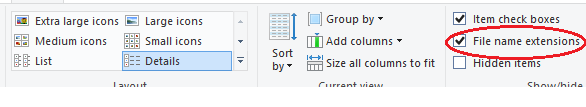
\includegraphics[width=.45\textwidth]{windowsView.png}}
\end{parbox}&\begin{parbox}{0.45\textwidth}{Save the Template as a .csv file, then change the extension from .csv to .lst. If the extension of the file is not shown, check the checkbox of "File name extensions" under View in your File Explorer.}
\end{parbox}\\
\hline
\begin{parbox}{0.45\textwidth}{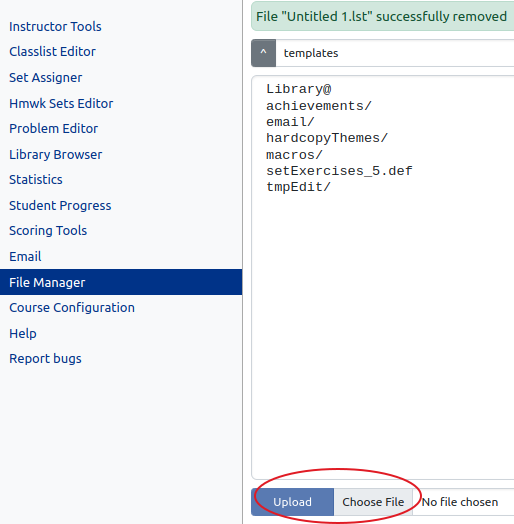
\includegraphics[width=0.45\textwidth]{fileManager.png}}
\end{parbox}&\begin{parbox}{0.45\textwidth}{In the course page on WeBWork, click File Manager in the navigation bar on the left, then upload the .lst file you just created.}
\end{parbox}\\
\hline
\begin{parbox}{0.45\textwidth}{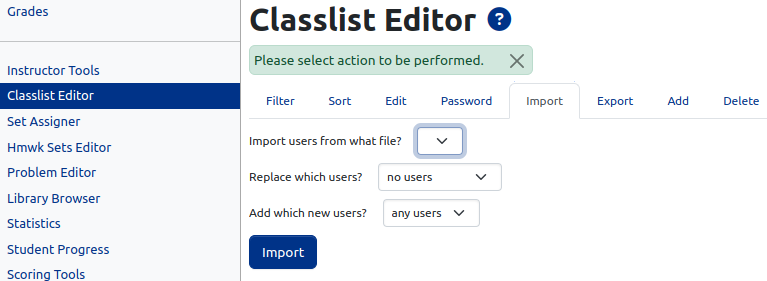
\includegraphics[width=.45\textwidth]{classlistEditor.png}}
\end{parbox}&\begin{parbox}{0.45\textwidth}{Lastly, click Classlist Editor, then import the students from the .lst file.}
\end{parbox}\\
\hline
\end{longtable}
}
\section{Import Grades from WeBWork to Canvas}
Assuming that you create the classlist according to the procedure in the last section, the process of importing grades back to Canvas is relatively easy.

{\centering
\begin{longtable}{|l|l|}
\hline
\begin{parbox}{0.45\textwidth}{\ }
\end{parbox}&\begin{parbox}{0.45\textwidth}{Download a copy of\\ Canvas\_Gradebook\_template.csv. In the following, we refer to this file as {\bf the Template}. }
\end{parbox}\\
\hline
\begin{parbox}{0.45\textwidth}{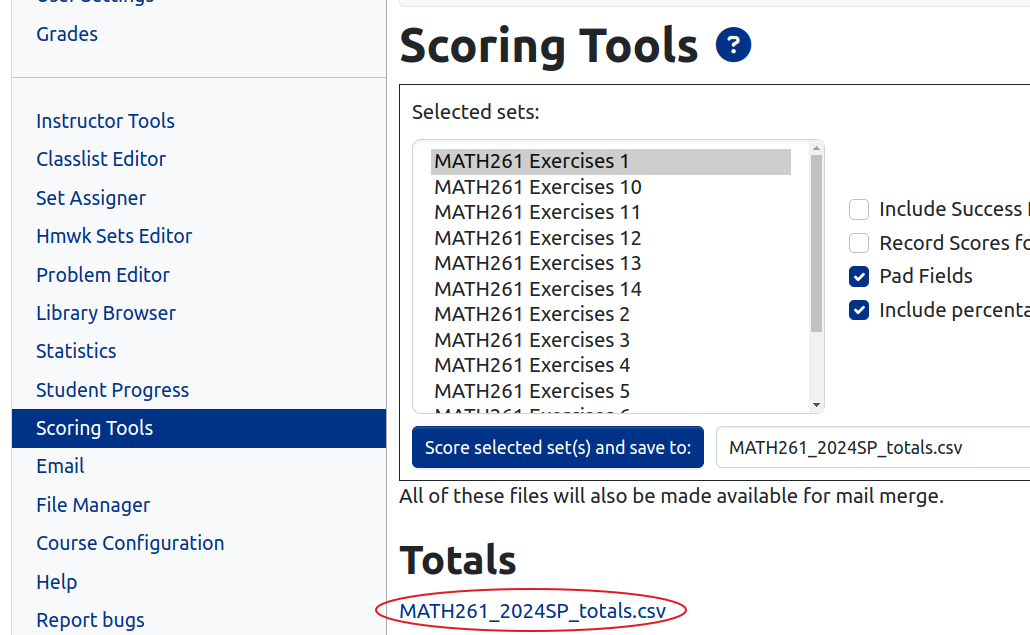
\includegraphics[width=.45\textwidth]{scoringTools.png}}
\end{parbox}&\begin{parbox}{0.45\textwidth}{In WeBWork, click Scoring Tools, then select the assignments you want to import, then click ``Score selected set(s) and save to'' after naming the file, then lastly click the file name below Totals to download the .csv file. }
\end{parbox}\\
\hline
\begin{parbox}{0.45\textwidth}{\ }
\end{parbox}&\begin{parbox}{0.45\textwidth}{Open both the Template and the WeBWork score .csv file with Microsoft Office Excel. Copy the following content from the score file to the Template:
\begin{itemize}
\item
Colume A (STUDENT ID) from Row 8 to Column B (ID) from Row 3. You have to make sure the student ID's are consistent with Canvas. We assume you follow the steps in Section 1 to get the student ID's.
\item Row 2(SET NAME) from Column G to Row 1 from Column F.
\item Row 6 (PROB VALUE) from Column G to Row 2 (Points Possible) from Column F.
\item Lastly, copy the scores and align them with the students and assignments.
\end{itemize}
}
\end{parbox}\\
\hline
\begin{parbox}{0.45\textwidth}{\includegraphics[width=.45\textwidth]{gradebookImport.png} }
\end{parbox}&\begin{parbox}{0.45\textwidth}{Save the template, then log in your Canvas, and click Import under Gradebook.}
\end{parbox}\\
\hline
\begin{parbox}{0.45\textwidth}{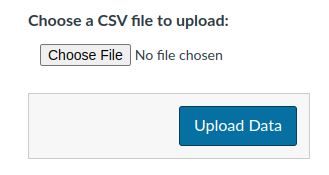
\includegraphics[width=.45\textwidth]{chooseScoreCSV.png} }
\end{parbox}&\begin{parbox}{0.45\textwidth}{Lastly, import the grades to Canvas with the populated template .csv file}
\end{parbox}\\
\hline
\begin{parbox}{0.45\textwidth}{\ }
\end{parbox}&\begin{parbox}{0.45\textwidth}{}
\end{parbox}\\
\hline
\end{longtable}
} 
\end{document}